%
% venn.tex
%


\documentclass{minimal}
\usepackage{tikz}

\begin{document}
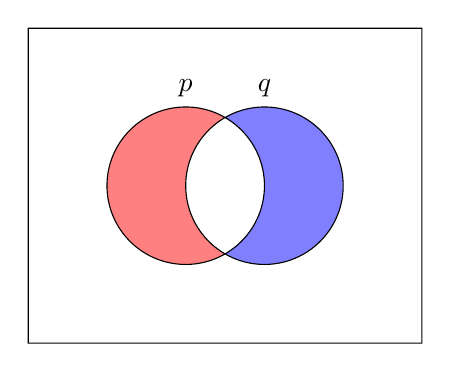
\begin{tikzpicture}[fill=gray]

% left hand
\scope
\clip (-2,-2) rectangle (2,2)
      (1,0) circle (1);
\fill[red!50] (0,0) circle (1);
\endscope

% right hand
\scope
\clip (-2,-2) rectangle (2,2)
      (0,0) circle (1);
\fill[blue!50] (1,0) circle (1);
\endscope

% outline
\draw (0,0) circle (1) (0,1)  node [text=black,above] {$p$}
      (1,0) circle (1) (1,1)  node [text=black,above] {$q$}
      (-2,-2) rectangle (3,2) ;


\end{tikzpicture}
\end{document}

